\documentclass[reprint, english, nofootinbib]{revtex4-2}

\usepackage{graphicx}
\usepackage{subfig}
\usepackage[colorlinks=true,urlcolor=blue,citecolor=blue]{hyperref}
\usepackage{physics}
\usepackage{amsmath}
\usepackage{amssymb}
\usepackage{amsbsy}
%\usepackage{bbold}
\usepackage{subfig}

\usepackage{blindtext}
\usepackage{tikzducks}
\usepackage{tikz}
\usepackage{pgfplots}
\usepackage{listings}

\graphicspath{{../figs/}}

\begin{document}
\title{Classification and Regression\\
\normalsize{From Linear and Logistic Regression to Neural Networks}}

\author{Nicholas Karlsen}
\affiliation{University of Oslo}
\author{Thore Espedal Moe}
\affiliation{University of Oslo}
\date{\today}

\begin{abstract}
\end{abstract}

\maketitle

\section{Introduction}

\section{Theory}
\subsection{Stochastic Gradient Descent}
\noindent
Consider a cost function in the form
\begin{equation}
    C(\pmb Y, \tilde{\pmb Y}(\pmb w)) = \frac{1}{N}\sum_{i=1}^{N}c_i(\pmb y_i, \tilde{\pmb y}(\pmb w)_i)
\end{equation}
which quantifies the error for some data set $\pmb Y = \left\{\pmb y_1, \dots, \pmb y_N\right\}$ with respect to a corresponding set of modeled data $\tilde{\pmb Y}(\pmb w) = \left\{\tilde{\pmb y_1}(\pmb w), \dots, \tilde{\pmb y}_N(\pmb w)\right\}$, where $\pmb w$ are denotes the free parameters of the model.

Since we can not in general expect to have a way of minimizing the cost analytically, we may in stead optimize it by gradient descent (GD), where the set of free parameters are incremented by
\begin{equation}
    \pmb w^{(k+1)} = \pmb w^{(k)} - \eta \nabla_{w}C\qty(\pmb Y, \tilde{\pmb Y}(\pmb w))
\end{equation}
until the cost function has reached a is found, where the parameter $\eta \in \mathbb R_{>0}$ denotes the learning rate. However, since we do not know a priori the shape of the space spanned by the cost function wrt. the parameters $\pmb w$, we can not tell whether the minima is indeed a global one, or simply a local minima.

One attempt at remedying this problem is the so-called \textit{Stochastic Gradient Descent} (SGD), in which stochasticity is introduced to the gradient descent by splitting the data set $\pmb Y$ into randomly sampled subsets $\pmb Y_{MB}$ called \textit{mini-batches} and then performing (GD) on each subset. Limiting the data-set in this way has the effect of "flattening" the space for each iteration, thus lessening the chance of getting stuck in local minima. This process is then repeated for multiple "epochs", where for each epoch we re-draw another random set of mini-batches from $\pmb Y$.



\begin{figure}[h!tb]
    \center
    \vspace{5mm} % To avoid touching the preceding text
    


\tikzset{every picture/.style={line width=0.75pt}} %set default line width to 0.75pt

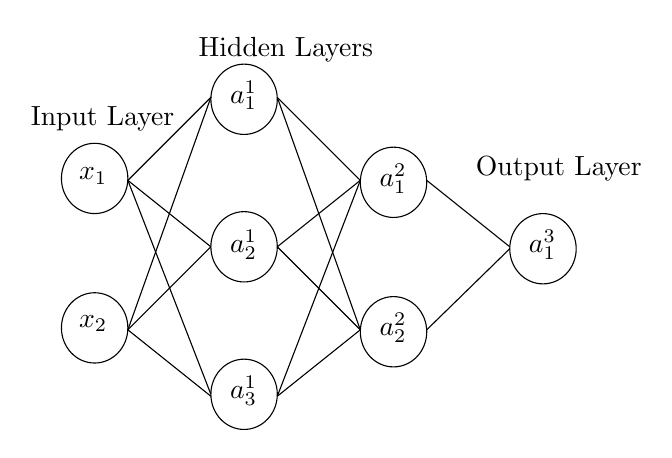
\begin{tikzpicture}[x=0.6pt,y=0.6pt,yscale=-1,xscale=1]
%uncomment if require: \path (0,484); %set diagram left start at 0, and has height of 484

%Flowchart: Connector [id:dp6019250960891445]
\draw  [fill={rgb, 255:red, 255; green, 255; blue, 255 }  ,fill opacity=1 ] (40,112.83) .. controls (40,101.14) and (48.95,91.67) .. (60,91.67) .. controls (71.05,91.67) and (80,101.14) .. (80,112.83) .. controls (80,124.52) and (71.05,134) .. (60,134) .. controls (48.95,134) and (40,124.52) .. (40,112.83) -- cycle ;
%Flowchart: Connector [id:dp8334547170271857]
\draw  [fill={rgb, 255:red, 255; green, 255; blue, 255 }  ,fill opacity=1 ] (40,202.83) .. controls (40,191.14) and (48.95,181.67) .. (60,181.67) .. controls (71.05,181.67) and (80,191.14) .. (80,202.83) .. controls (80,214.52) and (71.05,224) .. (60,224) .. controls (48.95,224) and (40,214.52) .. (40,202.83) -- cycle ;
%Flowchart: Connector [id:dp7153685420206096]
\draw  [fill={rgb, 255:red, 255; green, 255; blue, 255 }  ,fill opacity=1 ] (130,65.17) .. controls (130,53.48) and (138.95,44) .. (150,44) .. controls (161.05,44) and (170,53.48) .. (170,65.17) .. controls (170,76.86) and (161.05,86.33) .. (150,86.33) .. controls (138.95,86.33) and (130,76.86) .. (130,65.17) -- cycle ;
%Flowchart: Connector [id:dp5622283646258179]
\draw  [fill={rgb, 255:red, 255; green, 255; blue, 255 }  ,fill opacity=1 ] (130,154) .. controls (130,142.31) and (138.95,132.83) .. (150,132.83) .. controls (161.05,132.83) and (170,142.31) .. (170,154) .. controls (170,165.69) and (161.05,175.17) .. (150,175.17) .. controls (138.95,175.17) and (130,165.69) .. (130,154) -- cycle ;
%Flowchart: Connector [id:dp16862921724788715]
\draw  [fill={rgb, 255:red, 255; green, 255; blue, 255 }  ,fill opacity=1 ] (130,242.83) .. controls (130,231.14) and (138.95,221.67) .. (150,221.67) .. controls (161.05,221.67) and (170,231.14) .. (170,242.83) .. controls (170,254.52) and (161.05,264) .. (150,264) .. controls (138.95,264) and (130,254.52) .. (130,242.83) -- cycle ;
%Flowchart: Connector [id:dp4149695521858179]
\draw  [fill={rgb, 255:red, 255; green, 255; blue, 255 }  ,fill opacity=1 ] (220,115.17) .. controls (220,103.48) and (228.95,94) .. (240,94) .. controls (251.05,94) and (260,103.48) .. (260,115.17) .. controls (260,126.86) and (251.05,136.33) .. (240,136.33) .. controls (228.95,136.33) and (220,126.86) .. (220,115.17) -- cycle ;
%Flowchart: Connector [id:dp840876892841651]
\draw  [fill={rgb, 255:red, 255; green, 255; blue, 255 }  ,fill opacity=1 ] (220,205.17) .. controls (220,193.48) and (228.95,184) .. (240,184) .. controls (251.05,184) and (260,193.48) .. (260,205.17) .. controls (260,216.86) and (251.05,226.33) .. (240,226.33) .. controls (228.95,226.33) and (220,216.86) .. (220,205.17) -- cycle ;
%Flowchart: Connector [id:dp10784935111712701]
\draw  [fill={rgb, 255:red, 255; green, 255; blue, 255 }  ,fill opacity=1 ] (310,155.17) .. controls (310,143.48) and (318.95,134) .. (330,134) .. controls (341.05,134) and (350,143.48) .. (350,155.17) .. controls (350,166.86) and (341.05,176.33) .. (330,176.33) .. controls (318.95,176.33) and (310,166.86) .. (310,155.17) -- cycle ;
%Straight Lines [id:da7667435970573455]
\draw    (80,114) -- (130,154) ;
%Straight Lines [id:da48448129133283535]
\draw    (170,154) -- (220,114) ;
%Straight Lines [id:da4471635916327932]
\draw    (260,114) -- (310,154) ;
%Straight Lines [id:da5105417767244789]
\draw    (80,204) -- (130,244) ;
%Straight Lines [id:da6281305874976782]
\draw    (170,154) -- (220,204) ;
%Straight Lines [id:da9404110386397875]
\draw    (260,204) -- (310,155.17) ;
%Straight Lines [id:da669909761533326]
\draw    (130,154) -- (80,204) ;
%Straight Lines [id:da03861624272354913]
\draw    (80,204) -- (130,64) ;
%Straight Lines [id:da7865539839743194]
\draw    (80,114) -- (130,64) ;
%Straight Lines [id:da006395151871996019]
\draw    (170,64) -- (220,114) ;
%Straight Lines [id:da6703248416054105]
\draw    (170,64) -- (220,204) ;
%Straight Lines [id:da568582824840071]
\draw    (170,244) -- (220,204) ;
%Straight Lines [id:da5603512527475397]
\draw    (170,244) -- (220,114) ;
%Straight Lines [id:da15589575659778376]
\draw    (80,114) -- (130,242.83) ;

% Text Node
\draw (49,105) node [anchor=north west][inner sep=0.75pt]    {$x_{1}$};
% Text Node
\draw (49,194) node [anchor=north west][inner sep=0.75pt]    {$x_{2}$};
% Text Node
\draw (140,52.33) node [anchor=north west][inner sep=0.75pt]    {$a^{1}_{1}$};
% Text Node
\draw (140,142.33) node [anchor=north west][inner sep=0.75pt]    {$a^{1}_{2}$};
% Text Node
\draw (140,230) node [anchor=north west][inner sep=0.75pt]    {$a^{1}_{3}$};
% Text Node
\draw (230,102.33) node [anchor=north west][inner sep=0.75pt]    {$a^{2}_{1}$};
% Text Node
\draw (230,192.33) node [anchor=north west][inner sep=0.75pt]    {$a^{2}_{2}$};
% Text Node
\draw (320,142.33) node [anchor=north west][inner sep=0.75pt]    {$a^{3}_{1}$};
% Text Node
\draw (20,68) node [anchor=north west][inner sep=0.75pt]   [align=left] {Input Layer};
% Text Node
\draw (288,98) node [anchor=north west][inner sep=0.75pt]   [align=left] {Output Layer};
% Text Node
\draw (185,35) node   [align=left] {\begin{minipage}[lt]{74.80000000000001pt}\setlength\topsep{0pt}
Hidden Layers
\end{minipage}};


\end{tikzpicture}

    \caption{\label{fig: NN Fig} Visual representation of a simple neural network with $2$ inputs, $2$ hidden layers with $3$, $2$ neurons respectively and an output layer with a single neuron.}
\end{figure}

\subsection{Neural Networks}
\noindent
Neural Networks are a class of algorithms in which a set of nodes, often referred to as Neurons, are connected as a weighted graph. Which as the name may suggests, aims to emulate behaviour similar to that of the human brain. Each of the nodes in this graph is then activated by an activation function, which takes the weighted input of all of its connected graphs like
\begin{equation}
    a = \sigma\qty(w_1 a_1' + w_2 a_2' + \dots + w_n a_n' + b)
\end{equation}
where $w_i$, $a_i'$ denotes the weights and activations of the connected nodes, and $sigma$ the activation function of the node, for which is chosen differently depending on the problem at hand. Lastly, we have also introduced a bias, $b$, which simply shifts the activation of the Node. In the very simple case where the activation function is chosen to be the identity function, the bias term simply reduces to being the intercept.

The simplest type of neural network is the \textit{Feed-Forward Neural Network}, which is a directed graph, consisting of layers where each neuron in the preceding layer is connected to each neuron in the following layer as depicted in Fig.~\ref{fig: NN Fig}, which is directed from left to right.

As the name may suggest, the input layer is where the input data starts out, before being fed forward through the hidden layers of the network, weighted in-between each node before it finally reaches the output layer, the final model. In a similar fashion to other methods of supervised learning, the neural network must first undergo a process of training to obtain

\subsubsection{Backpropagation}
\noindent
Start by computing the response of each of the neurons in the network by the Feed-Forward algorithm, starting with the first hidden layer
\begin{align}\label{eqn: FeedForward Initial}
    \begin{split}
        z^1_j &= w^1_{jk}X_k + b^1_j \\
        a^1_j &= \sigma(z^1_j)
    \end{split}
\end{align}
where we adopt the Einstein summation convention by summing over repeated indices.
We then compute
\begin{align}
    \begin{split}
        z^l_{j} &= w^l_{jk}a^{l-1}_k + b^l_j \\
        a^l_{j} &= \sigma(z^l_{j})
    \end{split}
\end{align}
for hidden layers $l = 2, \dots, L$. Then, for the output layer we compute
\begin{align}
    \begin{split}
        z^{L}_j &= w^{L}_{jk}a^{L-1}_k + b^{L}_j \\
        a^{L}_j &= \tilde\sigma(z^{L}_j)
    \end{split}
\end{align}
where $a^{L}_j$ is the predicted response, and $\tilde\sigma$ is the activation function for the output layer, which may differ from the activation function of the hidden layers.

We then compute the error of the output as
\begin{equation}
    \delta^{L}_j = \pdv{C}{a^{L}_{j}} \odot \tilde\sigma'(z^{L}_j)
\end{equation}
and backpropagate the error like
\begin{equation}
    \delta^{l}_j = \qty(\delta^{l+1}_{k}\qty(w^{l+1})^T_{kj}) \odot \sigma'(z^l_j)
\end{equation}
for all $l = L-1, \dots, 1$.

We may then easily compute the gradients of the cost function wrt. the weights \& biases as

\begin{align}
    \begin{split}
        \pdv{C}{w_{jk}^l} &= \delta_j^l a^{l-1}_k \\
        \pdv{C}{b^l_j} &= \delta_j^l
    \end{split}
\end{align}
which are then used to update the weights and biases via gradient descent. Notably, we have not justified in any detail as to why this algorithm works, for which we refer the reader to \textcite{Mehta_2019}, \textcite{hastie}, or any other text on machine learning. However, in summary, it is all made possible by utilizing the chain rule.

\subsubsection{Backpropagation with mini-batches}
\noindent
In order to efficiently perform backpropagation simultaneously across several inputs at once, we need to slightly adjust our algorithm such that we may take advantage of the fast and efficient linear algebra libraries that are available, like i.e Numpy.

We then structure our input and output matrices adhering to the row-major storage of Numpy arrays by letting $X\in[M\times P], \enspace Y\in[M\times Q]$ where $M$ denotes the number of data points in the mini-batch and $P, Q$ the dimensionality of the input and output respectively. Explicitly, our data then undergoes the structure change

\begin{equation}
    X = \qty[
    \begin{matrix}
        X_1 \\ \vdots \\ X_P
    \end{matrix}
    ] \rightarrow
    X = \qty[
    \begin{matrix}
        X_{11} & \dots & X_{1P} \\
                 & \vdots&          \\
        X_{M1} & \dots & X_{MP}
    \end{matrix}
    ]
\end{equation}
similarly, we let $z^l_j \rightarrow z^l_{mj}$ and $a^l_{j}\rightarrow a^l_{mj}$ such that they are in accordance with $X$ and $Y$.

In order to adhere to this new form, we transpose Eqn.~\ref{eqn: FeedForward Initial} which yields
\begin{equation}
    w_{jk}X_K \rightarrow \qty(w_{jk}X_k)^T = X_k^T \qty(w^1)^T_{kj}
\end{equation}
Thus, we may write the initial step as
\begin{align}
    \begin{split}
        z^1_{mj} &= X_{mk}\qty(w^{1})^T_{kj} + b^1_j \\
        a^1_{mj} &= \sigma\qty(z^1_{mj})
    \end{split}
\end{align}
where the transposed bias is implicitly\footnote{Matching the behaviour of Numpys addition operator} added element-wise to each row in the resultant matrix. In a similar fashion, we feed forward for $l = 2, \dots L-1$, the last hidden layer as
\begin{align}
    \begin{split}
        z^l_{mj} &= a^{l-1}_{mk}\qty(w^l)^T_{kj} + b^L_j \\
        a^l_{mj} &= \sigma(z^l_{mj})
    \end{split}
\end{align}
and for the output layer
\begin{align}
    \begin{split}
        z^L_{mj} &= a^{L-1}_{mk}\qty(w^L)^T_{kj} + b^L_j \\
        a^L_{mj} &= \tilde\sigma\qty(z^L_{mj})
    \end{split}
\end{align}
Then, we compute the error of the output error as
\begin{equation}
    \delta^L_{mj} = \pdv{C}{a^L_{mj}} \odot \tilde\sigma'(z^L_{mj})
\end{equation}
which we then backpropagate throughout the layers for $l = L-1, \dots 1$
\begin{equation}
    \delta^{l}_{mj} = \delta^{l+1}_{mk}w^{l+1}_{kj} \odot \sigma'(z^l_{mj})
\end{equation}
and finally for the output layer. We the compute the derivatives of the cost functions wrt. the weights and biases for the input layer
\begin{align}
    \begin{split}
        \pdv{C}{w^{1}_{jk}} &= \qty(\delta^1)^T_{jm} X_{mk} \\
        \pdv{C}{b^1_{j}} &= \sum_m \delta^1_{mj}
    \end{split}
\end{align}
and similarly for layers $l = 2, \dots, L$ as
\begin{align}
    \begin{split}
        \pdv{C}{w^{l}_{jk}} &= \qty(\delta^1)^T_{jm} a^l_{mk} \\
        \pdv{C}{b^l_{j}} &= \sum_m \delta_{mj}
    \end{split}
\end{align}
The derivatives are then used to update the weights and biases by gradient descent in the usual way.

\subsubsection{Considerations when fitting Neural Networks}


\begin{table*}[]
\caption{\label{tab: activation functions}Various Activation functions used in Neural Networks}
\setlength{\tabcolsep}{20pt}
\renewcommand{\arraystretch}{2.5}
\begin{tabular}{llll}
    Name & Activation Function & Derivative & Range \\
    \hline\hline
    Identity &
    $\sigma(x) = x$  &
    $\sigma'(x) = 1$ &
    $(-\infty, \infty)$
    \\ \hline
    Sigmoid &
    $\sigma(x) = \frac{1}{1 + e^{-x}}$  &
    $\sigma'(x) =\sigma(x)\qty(1-\sigma(x))$ &
    $(0, 1)$
    \\ \hline
    Tanh &
    $\sigma(x) = \tanh(x)$  &
    $\sigma'(x) =  1 - \tanh^2(x)$ &
    $(0, 1)$
    \\ \hline
    ReLU    &
    $\sigma(x) = \left\{\begin{matrix}0 & \text{for } x \leq 0 \\ x & \text{for } 0 < x\end{matrix}\right.$ &
    $\sigma'(x) = \left\{\begin{matrix}0 & \text{for } x \leq 0 \\ 1 & \text{for } 0 < x\end{matrix}\right.$ &
    $[0, \infty)$
    \\ \hline
    LeakyReLU &
    $\sigma(x) = \left\{\begin{matrix}0.01x & \text{for } x \leq 0 \\ x & \text{for } 0 < x\end{matrix}\right.$ &
    $\sigma'(x) = \left\{\begin{matrix}0.01 & \text{for } x \leq 0 \\ 1 & \text{for } 0 < x\end{matrix}\right.$ &
    $(-\infty, \infty)$
    \\ \hline
\end{tabular}
\end{table*}



\subsection{Logistic Regression}
\noindent
As opposed to linear regression where the aim is to project data-points into some linear basis as to model some continuous function, logistic regression instead aims to project data unto some binary response. This may in turn be used classify whether or not some particular data point fits into some category. Thus, we wish to fit our data unto some function $f : \mathbb R \rightarrow [0, 1]$.
\begin{figure}[h!tb]
    \center
    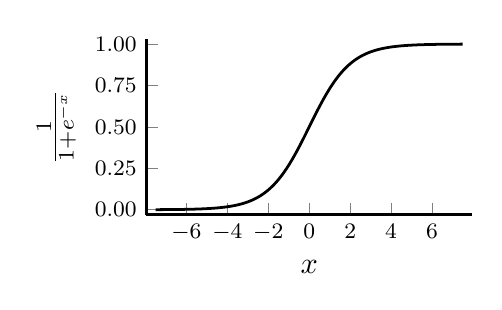
\begin{tikzpicture}[]
\begin{axis}[
  height = {38.1mm},
  ylabel = {$\frac{1}{1 + e^{-x}}$},
  xmin = {-7.95},
  xmax = {7.95},
  ymax = {1.029414054644861},
  xlabel = {$x$},
  unbounded coords=jump,scaled x ticks = false,xlabel style = {font = {\fontsize{11 pt}{14.3 pt}\selectfont}, color = {rgb,1:red,0.00000000;green,0.00000000;blue,0.00000000}, draw opacity = 1.0, rotate = 0.0},xmajorgrids = false,xtick = {-6.0,-4.0,-2.0,0.0,2.0,4.0,6.0},xticklabels = {$-6$,$-4$,$-2$,$0$,$2$,$4$,$6$},xtick align = inside,xticklabel style = {font = {\fontsize{8 pt}{10.4 pt}\selectfont}, color = {rgb,1:red,0.00000000;green,0.00000000;blue,0.00000000}, draw opacity = 1.0, rotate = 0.0},x grid style = {color = {rgb,1:red,0.00000000;green,0.00000000;blue,0.00000000},
draw opacity = 0.1,
line width = 0.5,
solid},axis x line* = left,x axis line style = {color = {rgb,1:red,0.00000000;green,0.00000000;blue,0.00000000},
draw opacity = 1.0,
line width = 1,
solid},scaled y ticks = false,ylabel style = {font = {\fontsize{11 pt}{14.3 pt}\selectfont}, color = {rgb,1:red,0.00000000;green,0.00000000;blue,0.00000000}, draw opacity = 1.0, rotate = 0.0},ymajorgrids = false,ytick = {0.0,0.25,0.5,0.75,1.0},yticklabels = {$0.00$,$0.25$,$0.50$,$0.75$,$1.00$},ytick align = inside,yticklabel style = {font = {\fontsize{8 pt}{10.4 pt}\selectfont}, color = {rgb,1:red,0.00000000;green,0.00000000;blue,0.00000000}, draw opacity = 1.0, rotate = 0.0},y grid style = {color = {rgb,1:red,0.00000000;green,0.00000000;blue,0.00000000},
draw opacity = 0.1,
line width = 0.5,
solid},axis y line* = left,y axis line style = {color = {rgb,1:red,0.00000000;green,0.00000000;blue,0.00000000},
draw opacity = 1.0,
line width = 1,
solid},    xshift = 0.0mm,
    yshift = 0.0mm,
    axis background/.style={fill={rgb,1:red,1.00000000;green,1.00000000;blue,1.00000000}}
,legend style = {color = {rgb,1:red,0.00000000;green,0.00000000;blue,0.00000000},
draw opacity = 1.0,
line width = 1,
solid,fill = {rgb,1:red,1.00000000;green,1.00000000;blue,1.00000000},fill opacity = 1.0,text opacity = 1.0,font = {\fontsize{8 pt}{10.4 pt}\selectfont}},colorbar style={title=},
  ymin = {-0.029414054644860983},
  width = {57.14999999999999mm}
]

\addplot+[
  color = {rgb,1:red,0.00000000;green,0.00000000;blue,0.00000000},
draw opacity = 1.0,
line width = 1,
solid,mark = none,
mark size = 2.0,
mark options = {
            color = {rgb,1:red,0.00000000;green,0.00000000;blue,0.00000000}, draw opacity = 1.0,
            fill = {rgb,1:red,0.00000000;green,0.00000000;blue,0.00000000}, fill opacity = 1.0,
            line width = 1,
            rotate = 0,
            solid
        },forget plot
] coordinates {
  (-7.5, 0.0005527786369235996)
  (-7.4, 0.000610879359434401)
  (-7.3, 0.0006750827306328381)
  (-7.2, 0.000746028833836697)
  (-7.1, 0.0008244246863982953)
  (-7.0, 0.0009110511944006454)
  (-6.9, 0.001006770820085637)
  (-6.8, 0.0011125360328603216)
  (-6.7, 0.0012293986212774202)
  (-6.6, 0.0013585199504289591)
  (-6.5, 0.0015011822567369917)
  (-6.4, 0.0016588010801744215)
  (-6.3, 0.0018329389424928053)
  (-6.2, 0.002025320389049882)
  (-6.1, 0.0022378485212763335)
  (-6.0, 0.0024726231566347743)
  (-5.9, 0.002731960763011059)
  (-5.8, 0.0030184163247084245)
  (-5.7, 0.0033348073074133443)
  (-5.6, 0.003684239899435989)
  (-5.5, 0.004070137715896128)
  (-5.4, 0.004496273160941178)
  (-5.3, 0.004966801650056961)
  (-5.2, 0.005486298899450404)
  (-5.1, 0.006059801491584117)
  (-5.0, 0.0066928509242848554)
  (-4.9, 0.007391541344281971)
  (-4.8, 0.008162571153159897)
  (-4.7, 0.009013298652847824)
  (-4.6, 0.009951801866904324)
  (-4.5, 0.01098694263059318)
  (-4.4, 0.012128434984274237)
  (-4.3, 0.013386917827664779)
  (-4.2, 0.014774031693273055)
  (-4.1, 0.016302499371440946)
  (-4.0, 0.01798620996209156)
  (-3.9, 0.01984030573407751)
  (-3.8, 0.021881270936130476)
  (-3.7, 0.024127021417669196)
  (-3.6, 0.026596993576865856)
  (-3.5, 0.02931223075135632)
  (-3.4, 0.032295464698450516)
  (-3.3, 0.03557118927263618)
  (-3.2, 0.039165722796764356)
  (-3.1, 0.043107254941086116)
  (-3.0, 0.04742587317756678)
  (-2.9, 0.05215356307841774)
  (-2.8, 0.057324175898868755)
  (-2.7, 0.06297335605699649)
  (-2.6, 0.06913842034334682)
  (-2.5, 0.07585818002124355)
  (-2.4, 0.08317269649392238)
  (-2.3, 0.09112296101485616)
  (-2.2, 0.09975048911968513)
  (-2.1, 0.10909682119561294)
  (-2.0, 0.11920292202211755)
  (-1.9, 0.13010847436299786)
  (-1.8, 0.14185106490048777)
  (-1.7, 0.15446526508353473)
  (-1.6, 0.16798161486607552)
  (-1.5, 0.18242552380635635)
  (-1.4, 0.19781611144141825)
  (-1.3, 0.2141650169574414)
  (-1.2, 0.23147521650098238)
  (-1.1, 0.24973989440488234)
  (-1.0, 0.2689414213699951)
  (-0.9, 0.289050497374996)
  (-0.8, 0.31002551887238755)
  (-0.7, 0.3318122278318339)
  (-0.6, 0.35434369377420455)
  (-0.5, 0.3775406687981454)
  (-0.4, 0.401312339887548)
  (-0.3, 0.425557483188341)
  (-0.2, 0.45016600268752216)
  (-0.1, 0.47502081252106)
  (0.0, 0.5)
  (0.1, 0.52497918747894)
  (0.2, 0.549833997312478)
  (0.3, 0.574442516811659)
  (0.4, 0.598687660112452)
  (0.5, 0.6224593312018546)
  (0.6, 0.6456563062257954)
  (0.7, 0.6681877721681662)
  (0.8, 0.6899744811276125)
  (0.9, 0.7109495026250039)
  (1.0, 0.7310585786300049)
  (1.1, 0.7502601055951177)
  (1.2, 0.7685247834990175)
  (1.3, 0.7858349830425586)
  (1.4, 0.8021838885585817)
  (1.5, 0.8175744761936437)
  (1.6, 0.8320183851339245)
  (1.7, 0.8455347349164652)
  (1.8, 0.8581489350995123)
  (1.9, 0.8698915256370021)
  (2.0, 0.8807970779778823)
  (2.1, 0.8909031788043871)
  (2.2, 0.9002495108803148)
  (2.3, 0.9088770389851438)
  (2.4, 0.9168273035060777)
  (2.5, 0.9241418199787566)
  (2.6, 0.9308615796566533)
  (2.7, 0.9370266439430035)
  (2.8, 0.9426758241011313)
  (2.9, 0.9478464369215823)
  (3.0, 0.9525741268224334)
  (3.1, 0.9568927450589139)
  (3.2, 0.9608342772032357)
  (3.3, 0.9644288107273639)
  (3.4, 0.9677045353015494)
  (3.5, 0.9706877692486436)
  (3.6, 0.973403006423134)
  (3.7, 0.9758729785823308)
  (3.8, 0.9781187290638694)
  (3.9, 0.9801596942659225)
  (4.0, 0.9820137900379085)
  (4.1, 0.9836975006285591)
  (4.2, 0.9852259683067269)
  (4.3, 0.9866130821723351)
  (4.4, 0.9878715650157257)
  (4.5, 0.9890130573694068)
  (4.6, 0.9900481981330957)
  (4.7, 0.990986701347152)
  (4.8, 0.9918374288468401)
  (4.9, 0.9926084586557181)
  (5.0, 0.9933071490757153)
  (5.1, 0.9939401985084158)
  (5.2, 0.9945137011005495)
  (5.3, 0.995033198349943)
  (5.4, 0.9955037268390589)
  (5.5, 0.995929862284104)
  (5.6, 0.9963157601005641)
  (5.7, 0.9966651926925867)
  (5.8, 0.9969815836752917)
  (5.9, 0.997268039236989)
  (6.0, 0.9975273768433653)
  (6.1, 0.9977621514787236)
  (6.2, 0.9979746796109501)
  (6.3, 0.9981670610575072)
  (6.4, 0.9983411989198255)
  (6.5, 0.998498817743263)
  (6.6, 0.9986414800495711)
  (6.7, 0.9987706013787226)
  (6.8, 0.9988874639671398)
  (6.9, 0.9989932291799144)
  (7.0, 0.9990889488055994)
  (7.1, 0.9991755753136017)
  (7.2, 0.9992539711661633)
  (7.3, 0.9993249172693672)
  (7.4, 0.9993891206405656)
  (7.5, 0.9994472213630764)
};

\end{axis}

\end{tikzpicture}


    \caption{The logistic function}
\end{figure}

\section{Results \& Discussion}
\section{Conclusion}

\onecolumngrid
\bibliography{bibfile}
\newpage
\twocolumngrid
\appendix
\end{document}
